\section{Performance scaling experiment} \label{sec:performance_scaling}

\subsection{Numerical results} \label{sec:numerical_results}

\begin{figure}[htbp]
    \centering
    \begin{subfigure}[t]{0.48\textwidth}
        \centering
        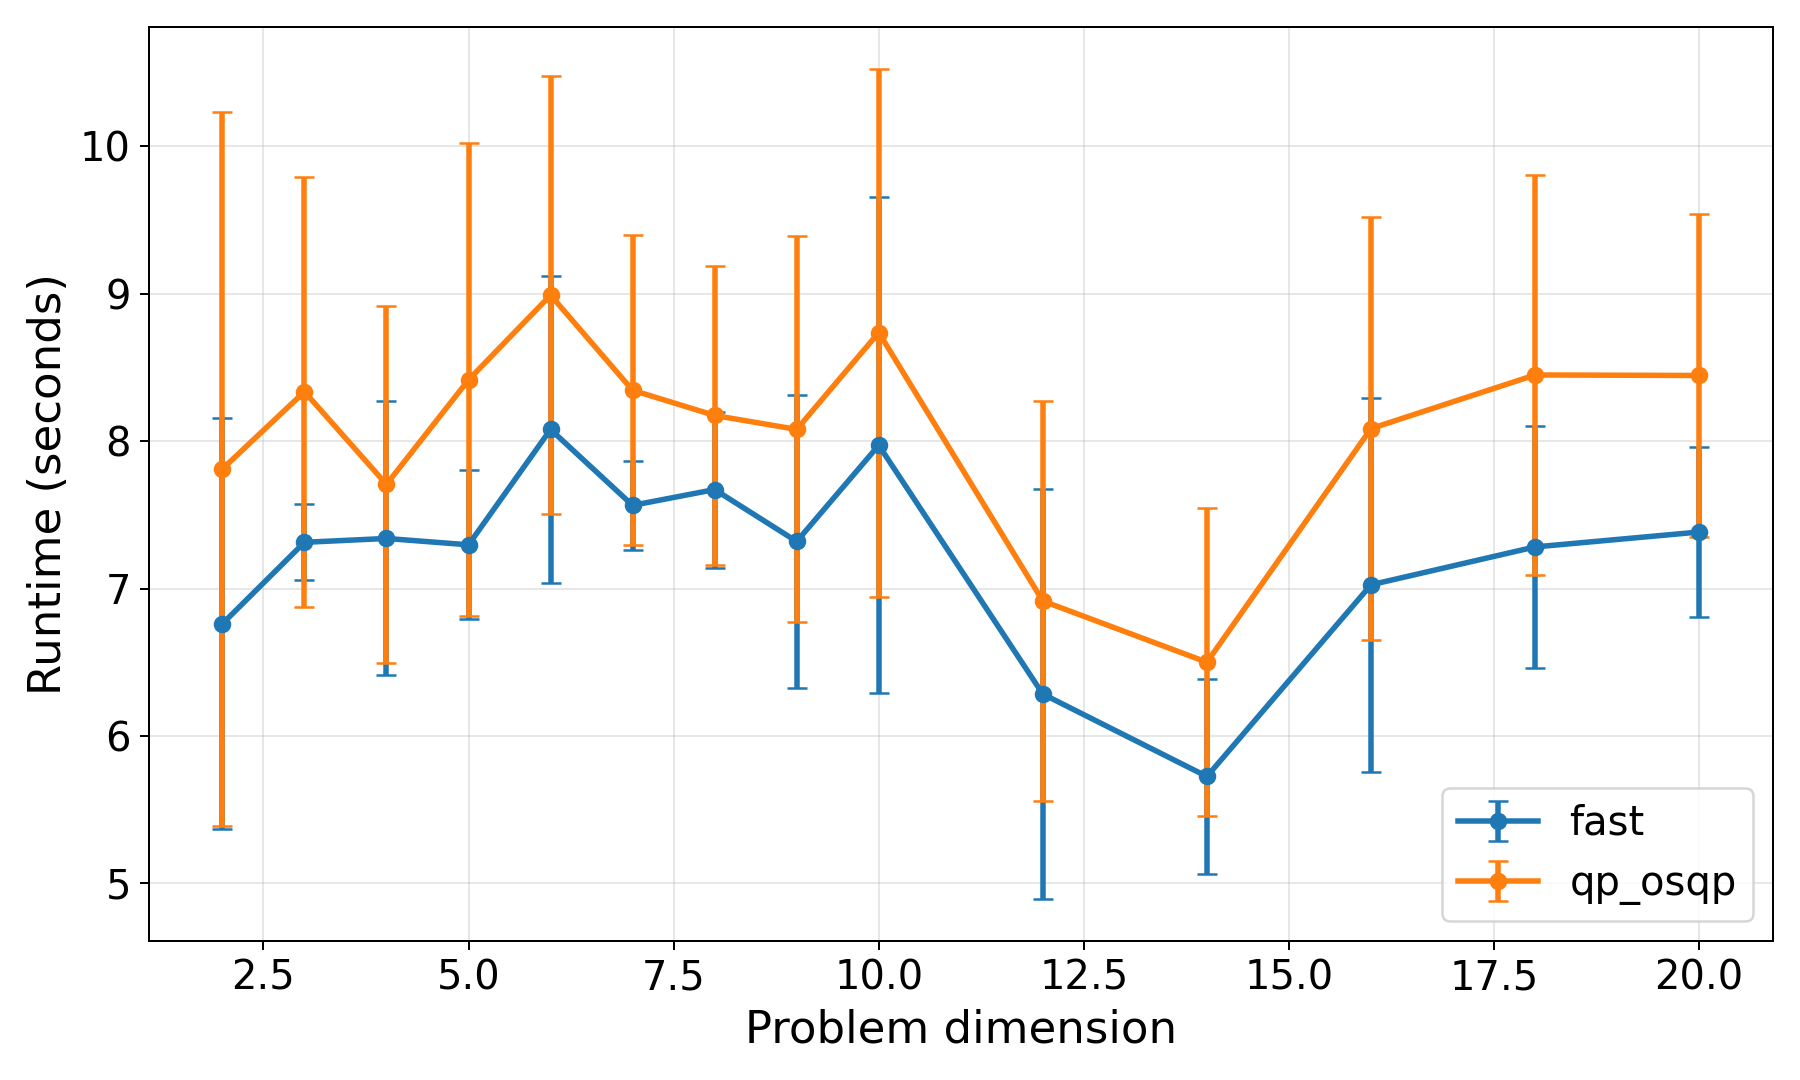
\includegraphics[width=\linewidth]{figures/solver_runtime_vs_dimension_component_TS=20260421_RegenTS=20260422-121449.png}
        \caption{Component TS}
        \label{fig:solver_runtime_component}
    \end{subfigure}\hfill
    \begin{subfigure}[t]{0.48\textwidth}
        \centering
        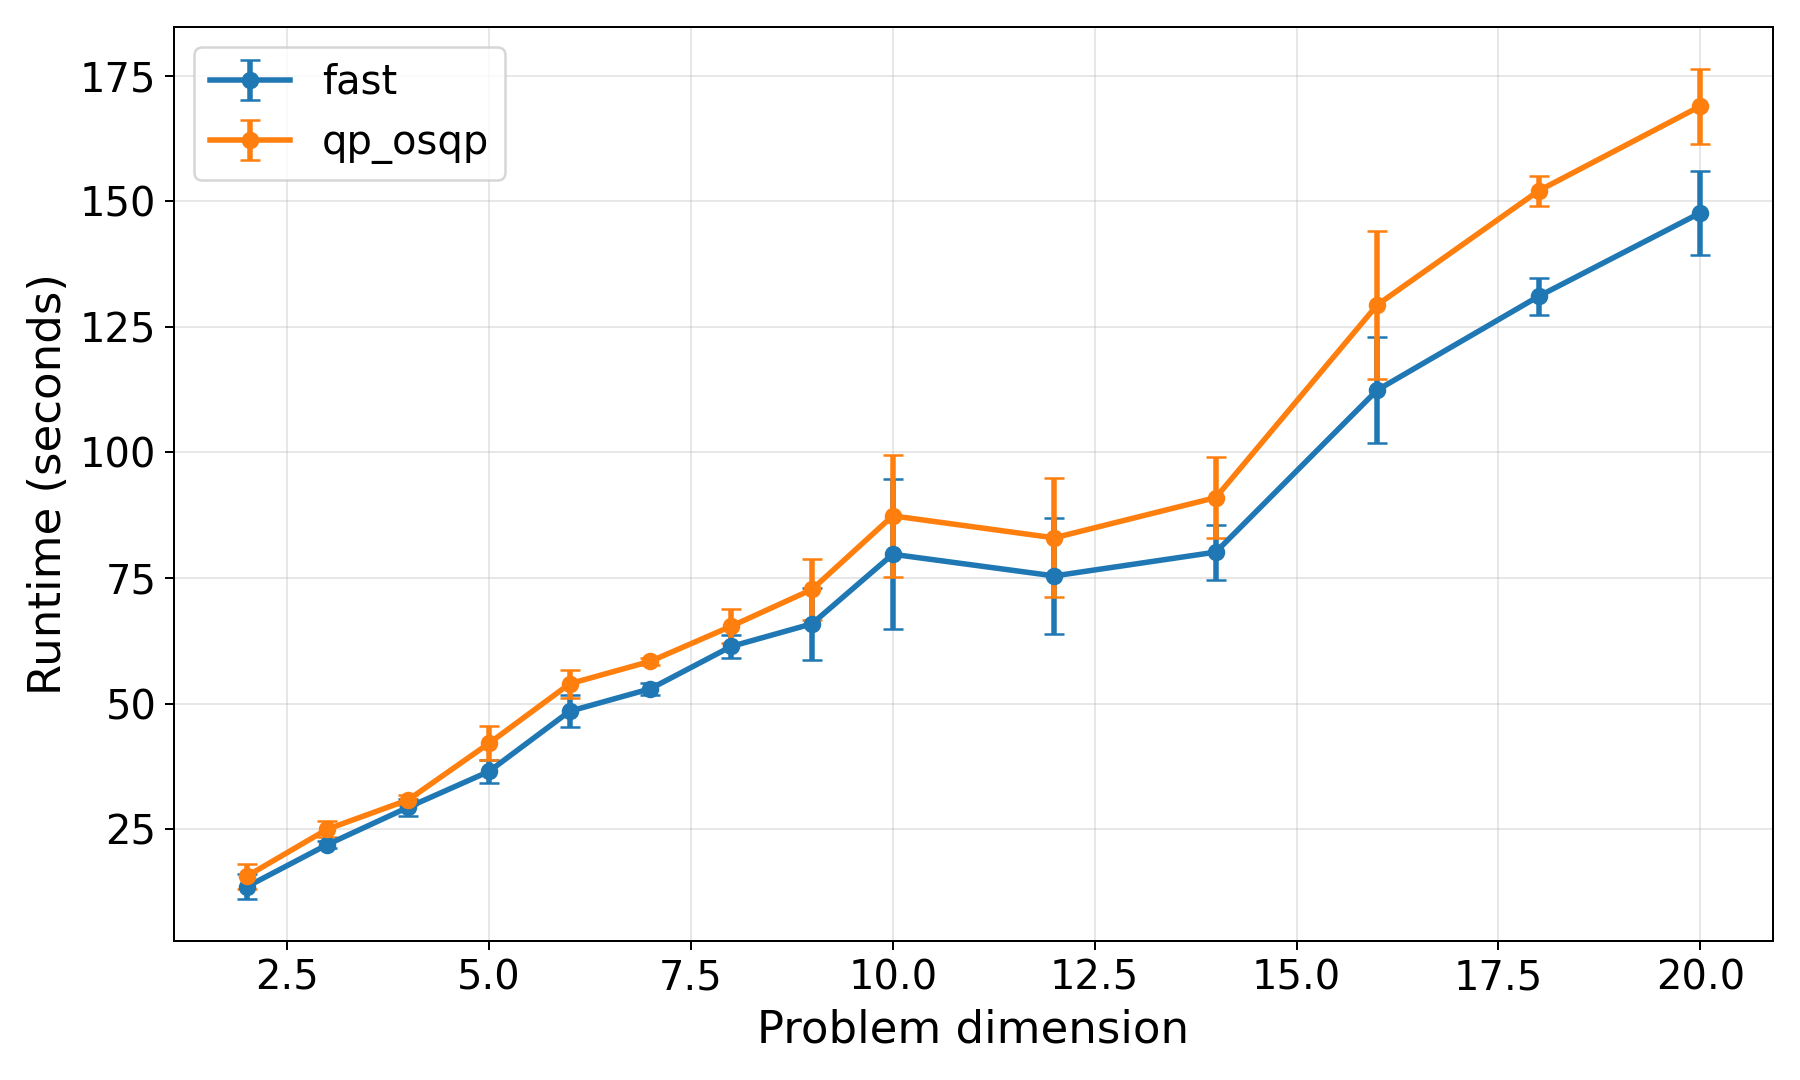
\includegraphics[width=\linewidth]{figures/solver_runtime_vs_dimension_fullmap_TS=20260421_RegenTS=20260422-121449.png}
        \caption{Full map}
        \label{fig:solver_runtime_fullmap}
    \end{subfigure}
    \caption{Solver runtime versus dimension for the two test settings.}
    \label{fig:solver_runtime_side_by_side}
\end{figure}

\begin{figure}[htbp]
    \centering
    \begin{subfigure}[t]{0.48\textwidth}
        \centering
        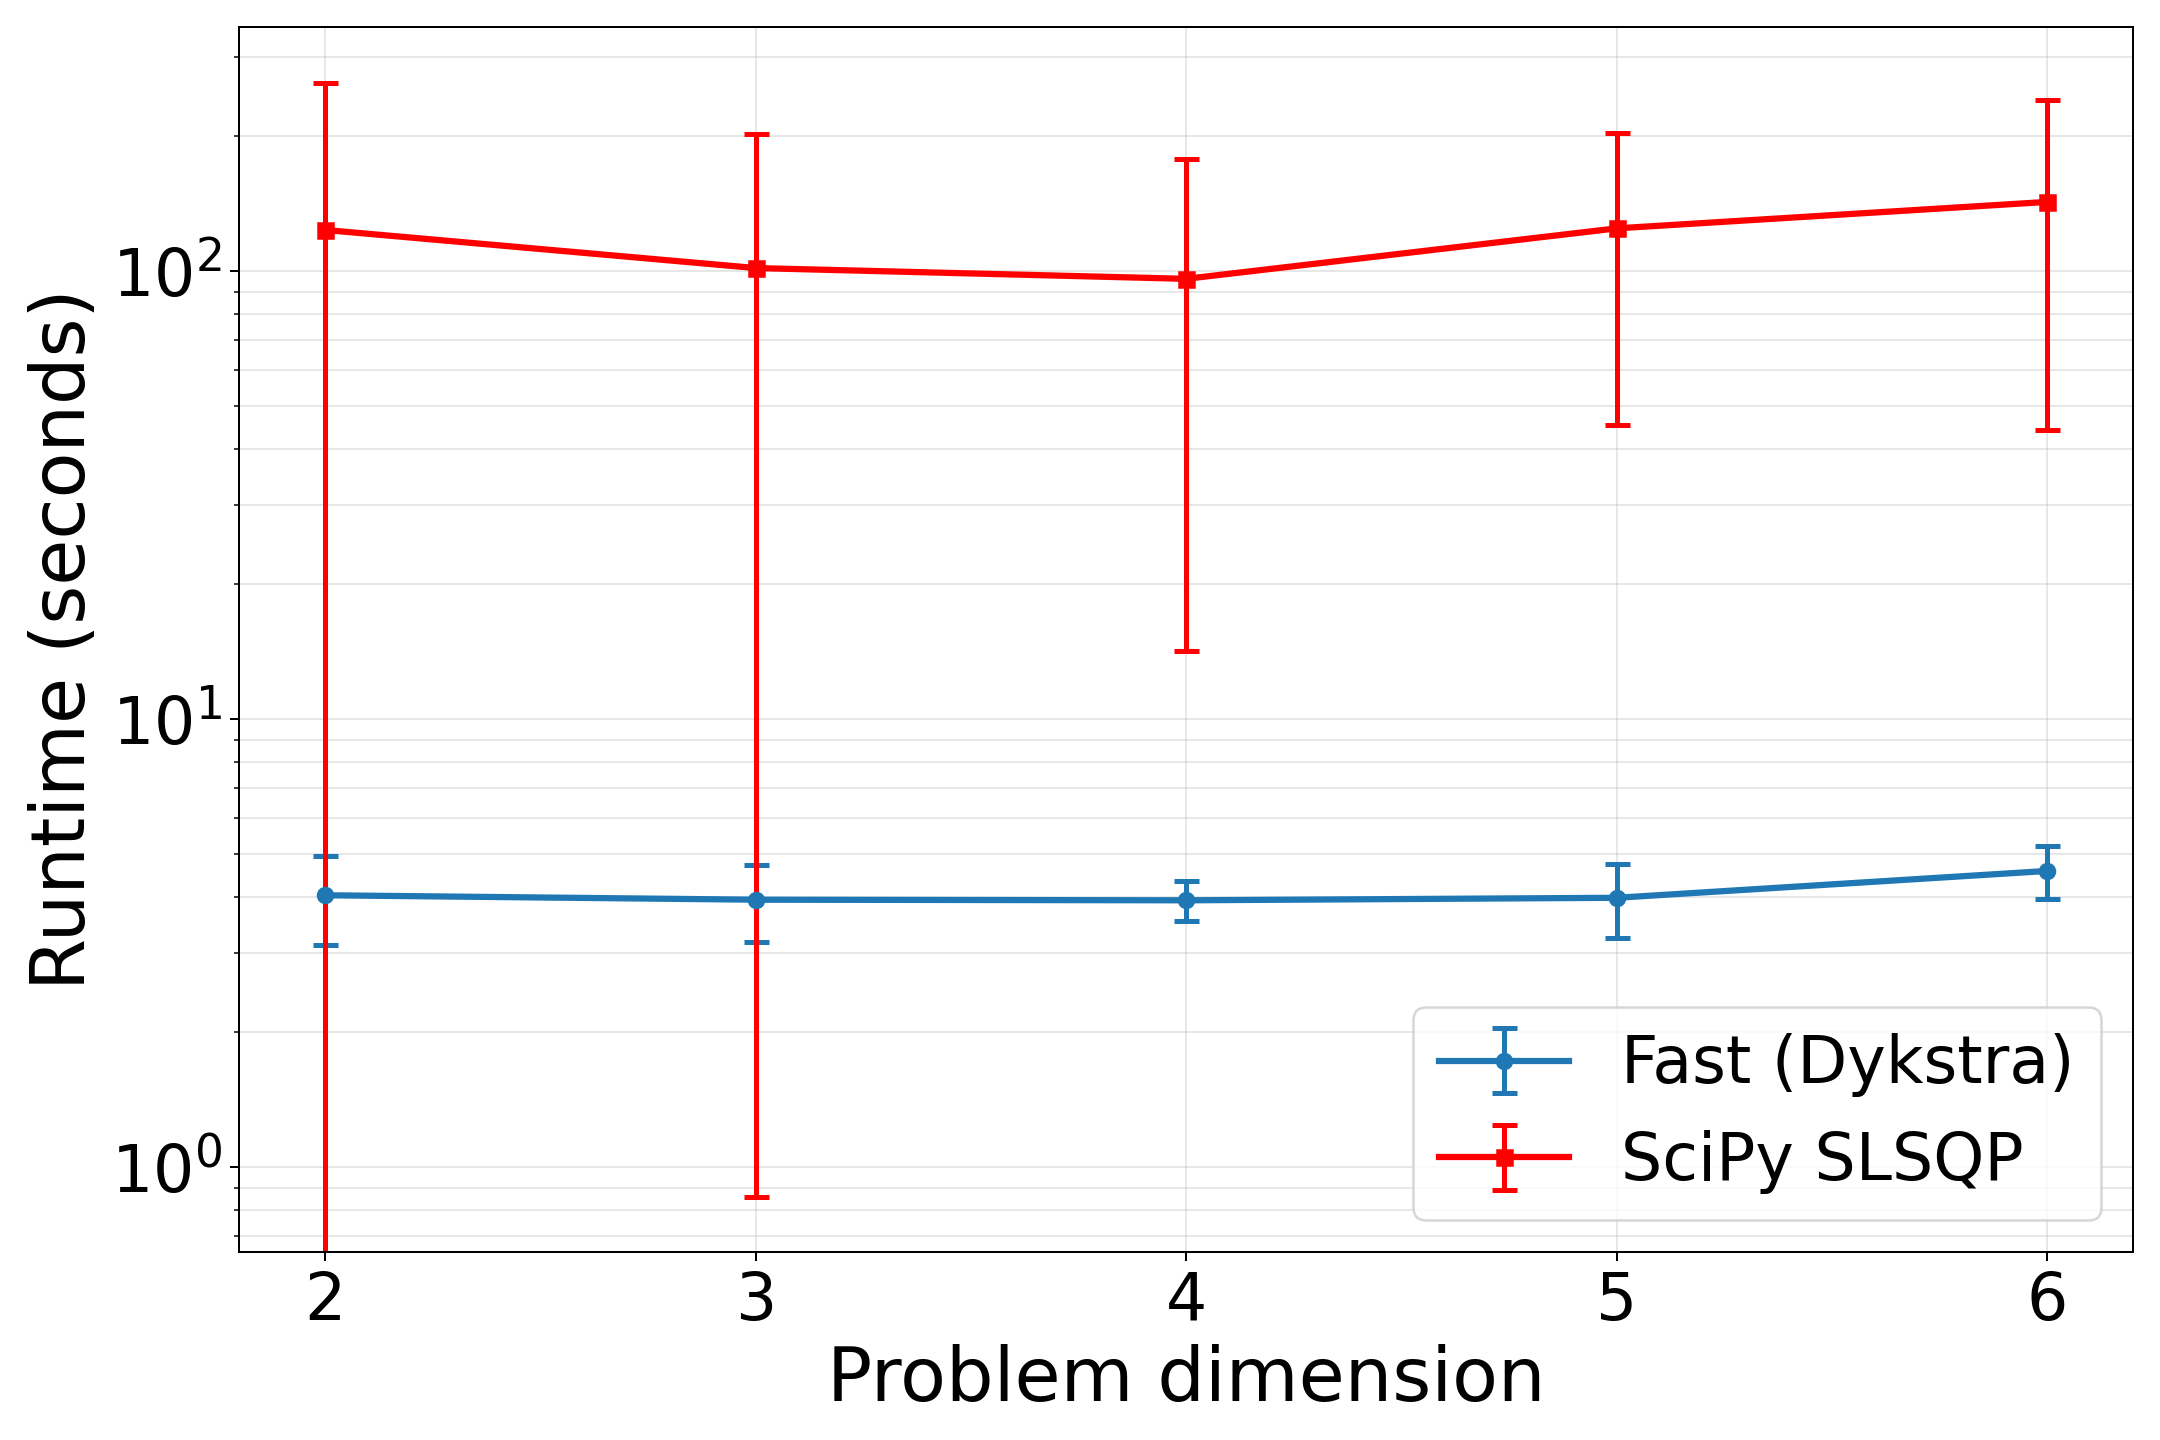
\includegraphics[width=\linewidth]{figures/fast_vs_scipy_component_log_scale.png}
        \caption{Component}
        \label{fig:fast_vs_scipy_component}
    \end{subfigure}\hfill
    \begin{subfigure}[t]{0.48\textwidth}
        \centering
        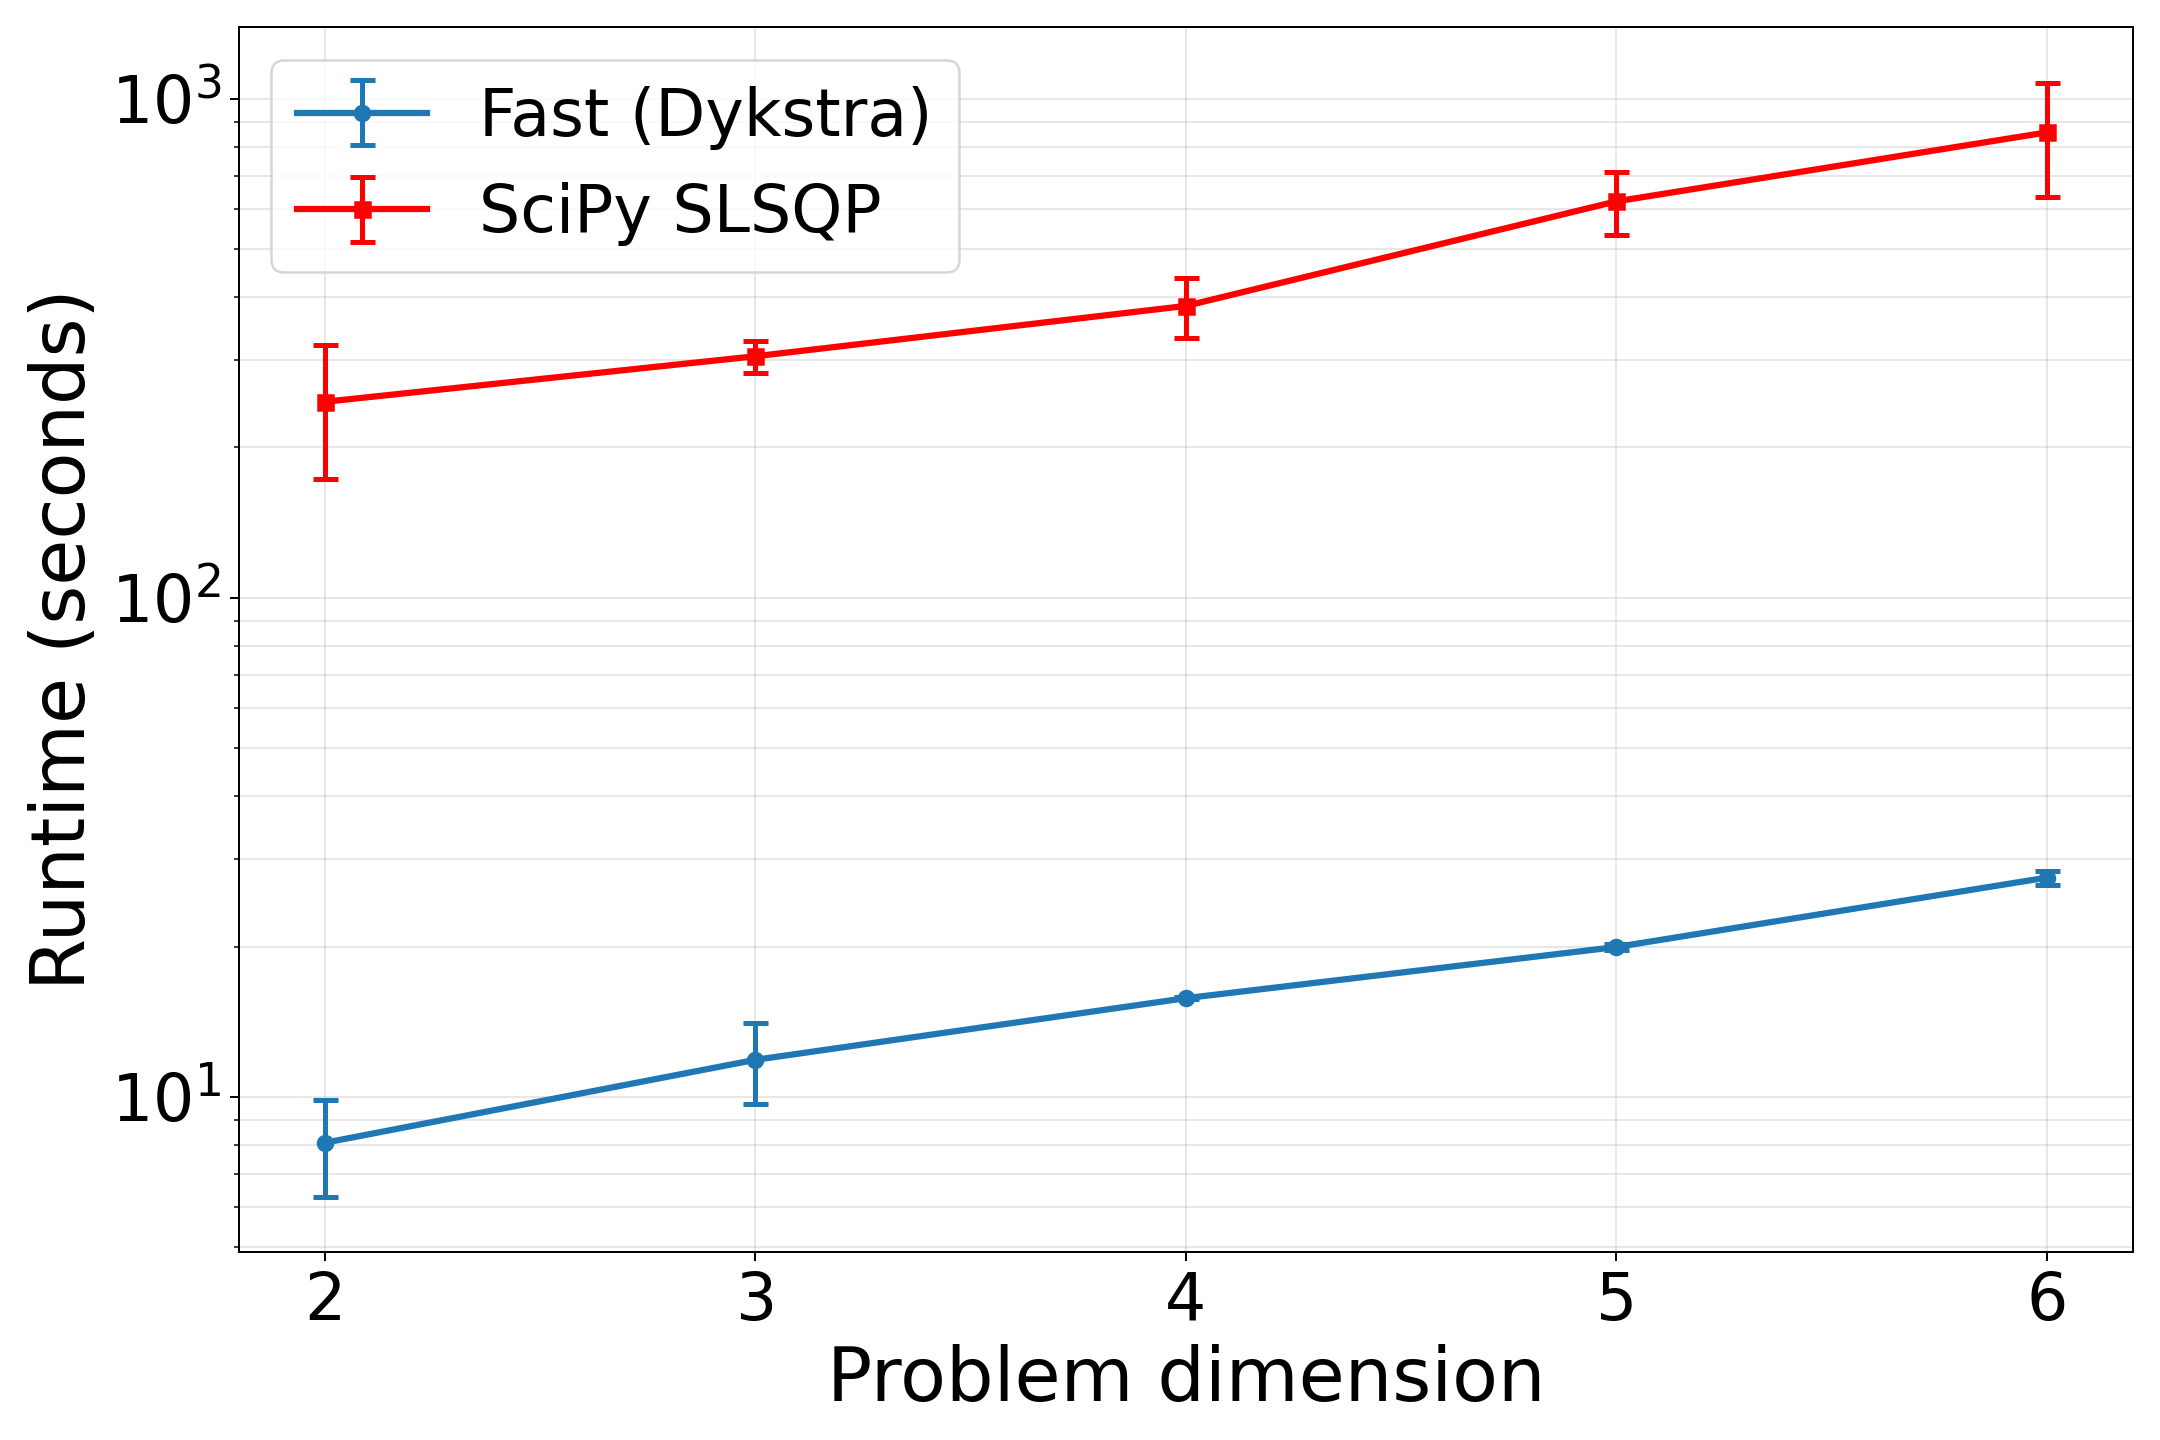
\includegraphics[width=\linewidth]{figures/fast_vs_scipy_overall_log_scale.png}
        \caption{Overall}
        \label{fig:fast_vs_scipy_overall}
    \end{subfigure}
    \caption{Runtime comparison between the fast solver and SciPy on a log scale.}
    \label{fig:fast_vs_scipy_side_by_side}
\end{figure}